\documentclass[conference]{IEEEtran}

\usepackage[T1]{fontenc}
\usepackage[utf8]{inputenc}
\usepackage{graphicx}
\usepackage{booktabs}
\usepackage{tabularx}
\usepackage{xcolor}
\usepackage{url}
\usepackage{cite}
\usepackage{hyperref}
\usepackage{tikz}
\usetikzlibrary{arrows.meta,positioning,shapes.geometric,shapes.multipart,fit}

\newcommand{\todo}[1]{\textcolor{red}{[TODO: #1]}}

\title{Brainrot Breakout: A Browser-Based Serious Game for Digital Well-Being Using Hand-Made Data Structures}

\author{
\IEEEauthorblockN{Samuel Navarro, Jos\'e Daza, Manuel Hormechea, Iv\'an Rivas}
\IEEEauthorblockA{\'Ultimo Scroll Studios, Universidad del Norte\\
Barranquilla, Colombia}
}

\begin{document}
\maketitle

\begin{abstract}
Excessive social media engagement and doomscrolling have raised concerns about digital well-being, while many interventions rely on reminders or explicit instruction. This work presents \emph{Brainrot Breakout}, a browser-based two-dimensional serious game that represents the trade-off between short-term relief and compulsive phone use through gameplay. The objective was to develop an accessible game that promotes reflection on healthier digital habits while applying data structures and abstract data types implemented from scratch. The project was developed in Godot 4.7 using GDScript and exported for web deployment. Its mechanics combine randomly positioned enemies, skill-based combat, six zones with boss encounters, accessibility settings, persistent records, and a leaderboard. Four hand-made abstract data types were implemented: \texttt{Lista}, \texttt{Cola}, \texttt{Leaderboard}, and \texttt{Registro}; the implementation uses linked-list, queue, and ordered-ranking structures. The software and its core mechanics were checked through code inspection. No empirical usability or performance outcome is claimed. The project demonstrates how data structures can support an interactive digital-well-being metaphor.
\end{abstract}

\begin{IEEEkeywords}
serious games, digital well-being, doomscrolling, data structures, abstract data types, accessibility, Godot
\end{IEEEkeywords}


\section{Introduction}
\label{p1-sec:intro}

Modern digital ecosystems are designed to sustain continuous engagement. Public health authorities have highlighted potential risks associated with social media exposure and youth mental health \cite{surgeon2023}. Platform features such as infinite feeds and algorithmic content delivery may reinforce habitual use and problematic engagement \cite{sharpe2026}. Doomscrolling, understood here as compulsive consumption of distressing digital content on mobile devices, is one manifestation of this pattern.

The problem addressed in this work is the limited availability of serious games that approach excessive social media use through implicit, mechanics-driven awareness rather than lectures or direct questions. Although usage limits and behavioral prompts can reduce time spent in selected applications, their effects on broader problematic-use measures may be limited \cite{mertens2026}. Serious games provide an alternative setting in which players can experience behavioral trade-offs through interaction \cite{andrew2023}. Accordingly, this project presents \emph{Brainrot Breakout}, a two-dimensional action game developed by Último Scroll Studios for the Data Structures I course at Universidad del Norte. Its central mechanic makes the virtual phone a source of short-term health recovery while increasing a dopamine meter and reducing visibility. The objective is to develop an accessible browser-based game that encourages reflection on healthy digital habits while integrating custom data structures and abstract data types into its architecture.

The remainder of this article is organized as follows. Section~\ref{p1-sec:contrib} presents the contributions, Section~\ref{p1-sec:related_work} reviews related work,
and Section~\ref{p1-sec:method} describes the methodology, including the system design, the data structures, the technological environment, and the use of AI tools.


\section{Contributions}
\label{p1-sec:contrib}

The contributions of this work are:
\begin{itemize}
\item \textbf{A playable metaphor for digital compulsion:} a risk--reward loop in which opening the phone restores health while increasing dopamine and blurring the screen.
\item \textbf{A six-zone action game:} six distinct boss encounters represent platform-related dynamics and require observation, timing, and tactical movement.
\item \textbf{Hand-made data abstractions:} four abstract data types (\texttt{Lista}, \texttt{Cola}, \texttt{Leaderboard}, and \texttt{Registro}) support wave progression, attack rotation, rotation of the pause-menu hints, ranking, and session persistence.
\item \textbf{Inclusive interaction options:} color-vision filters, independent audio buses, video blocking, two control schemes, and automatically activated touch controls.
\item \textbf{A browser-deployable implementation:} the game was exported from Godot for web execution, with local persistence for settings, records, and leaderboard entries.
\item \textbf{A documented requirements framework:} functional and non-functional requirements organized with FURPS+ guide the implementation and review of the game.
\end{itemize}

\section{Related Work}
\label{p1-sec:related_work}

Digital interventions targeting excessive social media consumption and problematic digital habits have gained significant scientific attention.
The United States Surgeon General issued an advisory highlighting how unchecked social media exposure poses substantial risks to youth mental health, associating heavy daily usage with higher rates of depressive symptoms and anxiety \cite{surgeon2023}.
To synthesize existing empirical findings, Sharpe et al. \cite{sharpe2026} conducted a systematic scoping review on doomscrolling, demonstrating consistent cross-sectional associations between compulsive negative media consumption and elevated distress, while emphasizing the critical scarcity of evaluated preventive interventions.

In response to these risks, several researchers have designed software-based interventions.
Mertens et al. \cite{mertens2026} evaluated \textit{Wellspent}, an iPhone application implementing behavioral nudges and self-set usage limits.
In a three-week randomized controlled trial with 70 participants, the authors observed a statistically significant reduction of 29 minutes per day in target application usage; however, the intervention did not produce significant reductions in broader self-reported problematic usage scale scores.
Building upon this trial dataset, Brockmeier et al. \cite{brockmeier2025} performed a secondary analysis examining psychological mechanisms, finding that stress reduction occurred primarily among users exhibiting higher baseline levels of problematic engagement.
Taking an educational prevention approach in vocational schools, Pietsch et al. \cite{pietsch2023} conducted a cluster-randomized controlled trial evaluating the mobile application \textit{Meine Zeit ohne}.
Their study demonstrated that voluntary two-week digital media abstinence commitments fostered measurable improvements in student health awareness across large cohort groups.

Alternative approaches leverage interactive narratives and serious games to promote digital well-being.
Andrew et al. \cite{andrew2023} conducted a systematic scoping review mapping serious health promotion games for adolescents, confirming their efficacy in transforming health attitudes while identifying a lack of gamified interventions addressing digital addiction.
Specifically targeting depressive symptoms, Sriwatanathamma et al. \cite{sriwatanathamma2023} developed \textit{BlueLine}, a visual novel integrating Cognitive Behavioral Therapy (CBT) through the ABCDE model.
The game constrained excessive virtual social interactions to sessions under one minute to simulate healthy boundaries, demonstrating how interactive narratives can deliver implicit therapeutic lessons.


Among the works reviewed here, a clear research gap remains.
Existing interventions rely primarily on external restrictive prompts, retrospective self-reporting, or linear narrative choices.
None of the reviewed systems integrates a real-time 2D action game loop where smartphone interaction functions as a risk-reward mechanic, coupled with implicit digital health awareness, inclusive visual design for colorblindness, and direct accessibility through standard web browsers.

\section{Methodology}
\label{p1-sec:method}

\subsection{Solution Alternatives}
Three alternatives were considered for the implementation:
\begin{itemize}
\item \textit{Alternative A: Python, Pygame, and pygbag.} This option offered a familiar language and game-library ecosystem, but required additional work for interface components, shaders, and touch input.
\item \textit{Alternative B: Java and libGDX.} This option offered a structured programming environment and game-development facilities, but web deployment and custom interface work introduced additional implementation effort.
\item \textit{Alternative C: Godot 4 and GDScript.} This option provided a game engine with web export, shader support, audio buses, and an integrated interface system \cite{godotdocs}.
\end{itemize}

\subsection{Evaluation and Selection}
The alternatives were compared using six criteria and weights. Table~\ref{p1-tab:eval} reports the scores recorded by the project team; the weighted totals are reproduced from that evaluation and have not been independently benchmarked. Alternative C was selected because it received the highest recorded weighted score and provided the web, shader, audio, and interface facilities required by the project.

\begin{table}[t]
\caption{Weighted evaluation of solution alternatives (scale 1--5).}
\label{p1-tab:eval}
\centering
\small
\begin{tabular}{p{3.15cm}cccc}
\toprule
\textbf{Criterion} & \textbf{Weight} & \textbf{A} & \textbf{B} & \textbf{C}\\
\midrule
Web and touch support & 0.25 & 3 & 2 & 5\\
Ease of implementation & 0.20 & 4 & 3 & 4\\
Performance & 0.15 & 3 & 4 & 4\\
Maintainability & 0.15 & 3 & 4 & 4\\
Development time & 0.15 & 4 & 2 & 4\\
Built-in UI, audio, and shaders & 0.10 & 2 & 2 & 5\\
\midrule
\textbf{Weighted total} & 1.00 & 2.85 & 2.80 & \textbf{4.35}\\
\bottomrule
\end{tabular}
\end{table}

\subsection{Functional Requirements}
Table~\ref{p1-tab:fr} presents the functional requirements used to guide implementation.

\begin{table*}[t]
\caption{Functional requirements of Brainrot Breakout.}
\label{p1-tab:fr}
\centering
\small
\begin{tabularx}{\textwidth}{@{}lX@{}}
\toprule
\textbf{ID} & \textbf{Requirement description}\\
\midrule
FR-01 & The system shall provide menu access to the game, arcade mode, settings, leaderboard, and help.\\
FR-02 & The player shall move and execute a slap attack (X key or right-click) that frees zombies within a frontal circular area; the freed count determines the score.\\
FR-03 & The player shall toggle a virtual phone: while open, health shall increase by 5 HP/s and dopamine by 8/s, movement shall slow, and the screen shall blur; while closed, dopamine shall decrease by 2/s.\\
FR-04 & The player shall lose and restart the current zone when health reaches zero or dopamine reaches 100.\\
FR-05 & The game shall randomize zombie spawn positions along the left, right, and bottom borders and the phone video content.\\
FR-06 & Gameplay shall require slap aiming, attack dodging, and decisions about when to open the phone.\\
FR-07 & The game shall provide six zones, progressive waves, and a boss every five waves, with stun vulnerability and phase transitions.\\
FR-08 & The system shall maintain a persistent leaderboard sorted by freed zombies and then by shorter completion time.\\
FR-09 & The system shall persist settings, the personal record, and leaderboard entries in local files.\\
FR-10 & The system shall provide color-vision filters, independent volume buses, video blocking, and two control schemes.\\
FR-11 & The system shall provide help screens, boss attack banners, and pause menus.\\
FR-12 & The game shall activate on-screen touch controls on touch-enabled devices.\\
FR-13 & The game shall provide audio feedback for gameplay, transitions, and victory.\\
FR-14 & Gameplay mechanics and states shall be represented graphically.\\
FR-15 & The core logic shall use at least three data-structure types and two hand-made abstract data types.\\
\bottomrule
\end{tabularx}
\end{table*}

\subsection{Non-Functional Requirements}
Non-functional requirements were organized using FURPS+ \cite{grady1987}. Table~\ref{p1-tab:nfr} summarizes the categories and constraints.

\begin{table*}[t]
\caption{Non-functional requirements structured using FURPS+.}
\label{p1-tab:nfr}
\centering
\small
\begin{tabularx}{\textwidth}{@{}p{2.45cm}lX@{}}
\toprule
\textbf{Category} & \textbf{ID} & \textbf{Description}\\
\midrule
Functionality & NFR-F1 & The game shall run locally without an external application server and shall store player nicknames locally.\\
Usability & NFR-U1 & Instructions and contextual guidance shall be accessible through the interface.\\
Usability & NFR-U2 & Audio-visual feedback shall communicate gameplay states.\\
Reliability & NFR-R1 & The game shall handle missing or malformed persistent-file entries without terminating the session.\\
Reliability & NFR-R2 & Nicknames shall be sanitized before persistence.\\
Performance & NFR-P1 & Browser frame rate shall be measured on desktop and mobile devices.\\
Supportability & NFR-S1 & Source files shall use modular organization, Spanish identifiers/comments, and a header comment.\\
Supportability & NFR-S2 & Version control shall follow GitHub Flow with pull-request integration.\\
Constraints (+) & NFR-C1 & The game shall be 2D, developed in Godot 4.7, exported for the web, and avoid explicit instructional questions.\\
\bottomrule
\end{tabularx}
\end{table*}

\subsection{Requirements Evaluation and Method}
The team used the functional and non-functional requirements as implementation and review criteria. The development process used GitHub Flow, pull requests, and a Trello task board; details are provided in Section~\ref{p3-sec:env}. The game was implemented in Godot 4.7 using GDScript. The requirements were checked through code inspection and gameplay evidence, without empirical usability or performance measurements. The FURPS+ categories cover functionality, usability, reliability, performance, supportability, and additional constraints. Nielsen's usability heuristics provide a complementary basis for interface inspection \cite{nielsen1994}.

A serious-game approach is consistent with research on game-based health promotion \cite{andrew2023}. The project did not claim a measured health outcome; its intended contribution was an interactive representation of the trade-off associated with repeated phone use.

% parte3.tex -- P3: System Design and Data Structures; Technological Environment and Development Process; Use of Artificial Intelligence Tools









\subsection{System Design and Data Structures}
\label{p3-sec:design}

The use cases of the system are modeled in Fig.~\ref{p3-fig:usecase}. The only actor is the player, who interacts with the main menu to start a new game (Zones 1 to 6 in sequence), to play a single zone in the arcade mode, to change the settings (volume, color-blindness filter, phone videos, and controls), to read the help, to view the leaderboard, and to exit the game (this option is hidden in the web build). Starting a new game and choosing an arcade zone both include \emph{Play zone}, which in turn includes \emph{Slap zombies}, the basic attack of the game. Four use cases extend \emph{Play zone}: opening the phone, pausing the game, retrying the zone after losing (the death screen), and fighting the boss, which appears every five waves. Saving a score extends the boss fight, because the nickname for the leaderboard is requested only after the final boss is defeated.

\begin{figure*}[t]
\centering
\includegraphics[width=0.7\textwidth]{casos_uso.pdf}
\caption{Use case diagram of Brainrot Breakout. Dashed arrows point from the including or extending use case as UML prescribes: \guillemotleft include\guillemotright\ from the base to the included case, \guillemotleft extend\guillemotright\ from the extension to the base.}
\label{p3-fig:usecase}
\end{figure*}

The architecture is organized in components, as Fig.~\ref{p3-fig:arch} shows. The main menu loads a zone scene, and each of the six zones (Table~\ref{p3-tab:zones}) is composed of a map, the player, a heads-up display (HUD), and a wave generator; the root script of the zone launches the waves and summons the boss. Five global singletons (autoloads) are available to every scene: \texttt{Ajustes} holds the volume buses (master, music, and effects), the color-blindness filter, the blocking of the phone videos, and the control scheme (arrows plus X, or WASD plus right click), and stores them in \texttt{ajustes.cfg}; \texttt{Pausa} manages the pause menu and its rotating hints; \texttt{Transicion} manages the fade transitions between zones; \texttt{MusicaGlobal} manages the music; and \texttt{Muerte} shows the death screen, which freezes the game and lets the player retry the zone or return to the menu. The player reads and writes the personal record and the elapsed time through \texttt{Registro}, and the menu displays the \texttt{Leaderboard}.

\begin{figure*}[t]
\centering
\resizebox{0.98\textwidth}{!}{%
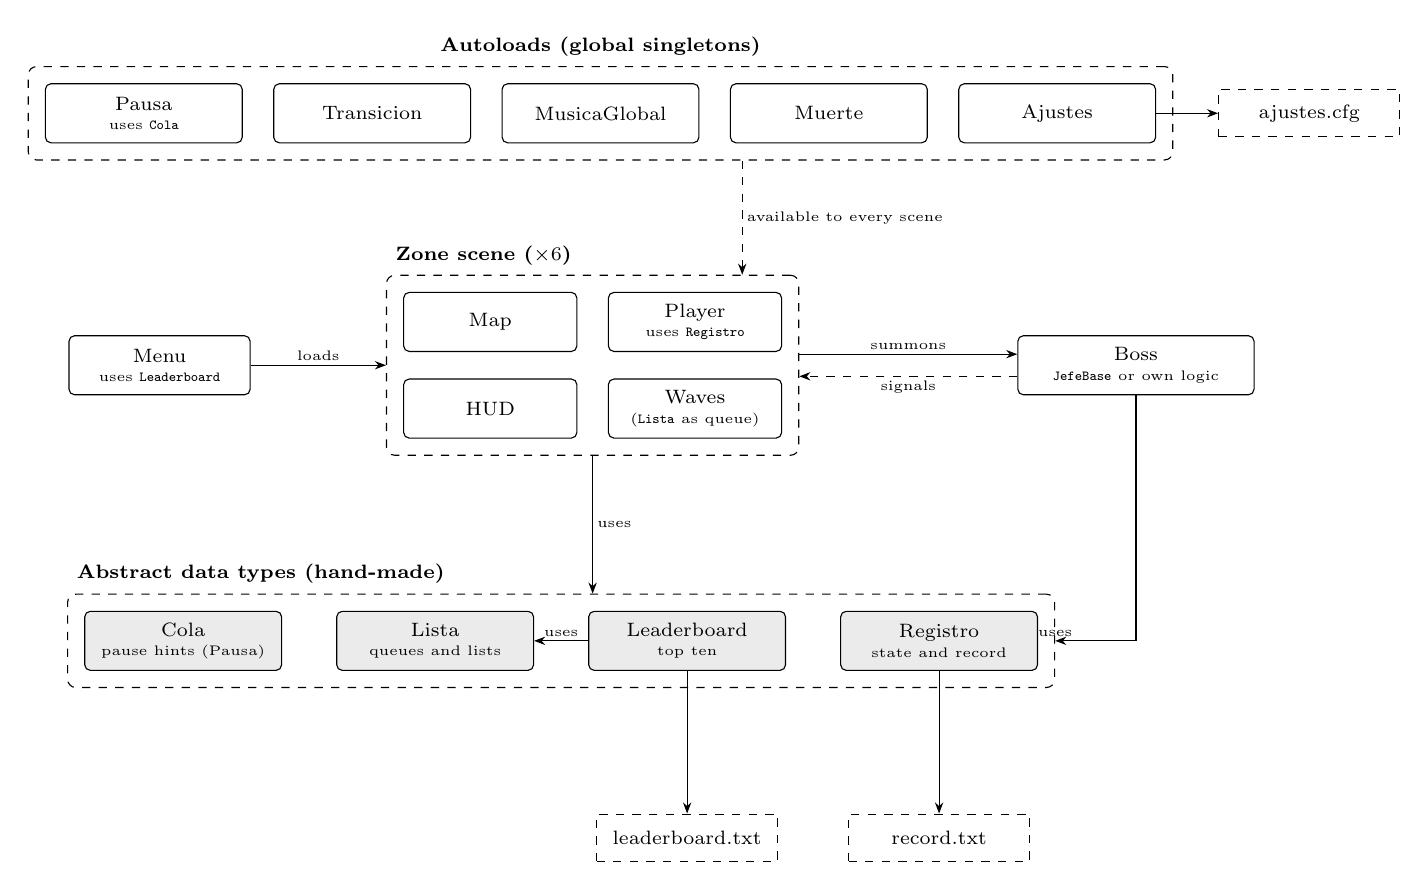
\begin{tikzpicture}[
  comp/.style={rectangle, draw, rounded corners=2pt, minimum width=2.5cm, minimum height=0.75cm, font=\scriptsize, align=center, inner sep=2pt},
  adt/.style={comp, fill=black!8},
  file/.style={rectangle, draw, dashed, minimum width=2.3cm, minimum height=0.6cm, font=\scriptsize, inner sep=2pt},
  grp/.style={draw, dashed, rounded corners=3pt, inner sep=6pt},
  use/.style={-{Stealth[length=4pt]}},
  lbl/.style={font=\tiny, inner sep=1.5pt}]
% autoloads
\node[comp] (pa) at (1.4,3.2) {Pausa\\[-1pt]{\tiny uses \texttt{Cola}}};
\node[comp] (tr) at (4.3,3.2) {Transicion};
\node[comp] (mu) at (7.2,3.2) {MusicaGlobal};
\node[comp] (mue) at (10.1,3.2) {Muerte};
\node[comp] (aj) at (13.0,3.2) {Ajustes};
\node[grp, fit=(pa)(tr)(mu)(mue)(aj), label={[font=\scriptsize\bfseries]above:Autoloads (global singletons)}] (auto) {};
\node[file] (cfg) at (16.2,3.2) {ajustes.cfg};
\draw[use] (aj) -- (cfg);
% menu, zone, boss
\node[comp, minimum width=2.3cm] (menu) at (1.6,0) {Menu\\[-1pt]{\tiny uses \texttt{Leaderboard}}};
\node[comp, minimum width=2.2cm] (mapa) at (5.8,0.55) {Map};
\node[comp, minimum width=2.2cm] (jug) at (8.4,0.55) {Player\\[-1pt]{\tiny uses \texttt{Registro}}};
\node[comp, minimum width=2.2cm] (hud) at (5.8,-0.55) {HUD};
\node[comp, minimum width=2.2cm] (ole) at (8.4,-0.55) {Waves\\[-1pt]{\tiny (\texttt{Lista} as queue)}};
\node[grp, fit=(mapa)(jug)(hud)(ole)] (zone) {};
\node[font=\scriptsize\bfseries, anchor=south west] at (zone.north west) {Zone scene ($\times 6$)};
\node[comp, minimum width=3.0cm] (boss) at (14.0,0) {Boss\\[-1pt]{\tiny \texttt{JefeBase} or own logic}};
\draw[use] (menu) -- (zone) node[midway, above, lbl] {loads};
\draw[use] ([yshift=4pt]zone.east) -- ([yshift=4pt]boss.west) node[midway, above, lbl] {summons};
\draw[use, dashed] ([yshift=-4pt]boss.west) -- ([yshift=-4pt]zone.east) node[midway, below, lbl] {signals};
\coordinate (dx) at (9.0,0);
\draw[use, dashed] (dx |- auto.south) -- (dx |- zone.north) node[midway, right, lbl] {available to every scene};
% abstract data types
\node[adt] (cola) at (1.9,-3.5) {Cola\\[-1pt]{\tiny pause hints (Pausa)}};
\node[adt] (lista) at (5.1,-3.5) {Lista\\[-1pt]{\tiny queues and lists}};
\node[adt] (lead) at (8.3,-3.5) {Leaderboard\\[-1pt]{\tiny top ten}};
\node[adt] (reg) at (11.5,-3.5) {Registro\\[-1pt]{\tiny state and record}};
\node[grp, fit=(cola)(lista)(lead)(reg)] (adts) {};
\node[font=\scriptsize\bfseries, anchor=south west] at (adts.north west) {Abstract data types (hand-made)};
\draw[use] (zone.south) -- (zone.south |- adts.north) node[midway, right, lbl] {uses};
\draw[use] (boss.south) |- (adts.east) node[above, lbl] {uses};
\draw[use] (lead.west) -- (lista.east) node[midway, above, lbl] {uses};
% files
\node[file] (lbt) at (8.3,-6.0) {leaderboard.txt};
\node[file] (rct) at (11.5,-6.0) {record.txt};
\draw[use] (lead.south) -- (lbt.north);
\draw[use] (reg.south) -- (rct.north);
\end{tikzpicture}}
\caption{Component architecture of Brainrot Breakout. Solid arrows indicate use or control flow, dashed arrows indicate global availability or signals, shaded boxes are the hand-made abstract data types, and dashed rectangles are files.}
\label{p3-fig:arch}
\end{figure*}

\begin{table}[t]
\caption{Zones and bosses of the game. Wave: wave at which the boss appears. HP/P2: boss health and health threshold of its second phase.}
\label{p3-tab:zones}
\centering
\footnotesize
\setlength{\tabcolsep}{3pt}
\begin{tabular}{clp{2.2cm}cc}
\toprule
\textbf{Zone} & \textbf{Setting} & \textbf{Boss} & \textbf{Wave} & \textbf{HP/P2} \\
\midrule
1 & Street & El Influencer Viral & 5 & 56/28 \\
2 & Social building & El Algoritmo & 10 & 60/30 \\
3 & Loading area & Capataz & 15 & 50/25 \\
4 & Elevator & Gemelo & 20 & 40/20 \\
5 & Laboratory & Dr. Dopamina & 25 & 24/12 \\
6 & Supercomputers & N\'ucleo-$\infty$ & 30 & 25/10 \\
\bottomrule
\end{tabular}
\end{table}

The bosses are the link between the zones and the data structures, and Fig.~\ref{p3-fig:classes} shows their classes together with those of the data structures. A boss receives damage only while it is stunned and enters a second phase when its health drops below a threshold (Table~\ref{p3-tab:zones}). The bosses of Zones 3 to 6 inherit from the base class \texttt{JefeBase}, which implements three states (intro, attacking, and stunned) and an attack queue with cooldowns. The bosses of Zones 1 and 2 have their own logic and follow the same contract with the rest of the game (the signals \texttt{vida\_cambiada} and \texttt{murio} and the method \texttt{recibir\_golpe}); for this reason the figure links them to \texttt{JefeBase} with a dashed arrow instead of an inheritance arrow. The final boss displays the victory screen and requests the name for the leaderboard. All graphics were drawn by code as placeholders that can be replaced by sprites.

\begin{figure*}[t]
\centering
\resizebox{0.98\textwidth}{!}{%
\begin{tikzpicture}[
  cls/.style={rectangle split, rectangle split parts=3, rectangle split part align={center,left,left}, draw, font=\scriptsize, align=left, inner sep=3pt, anchor=north},
  cls2/.style={cls, rectangle split parts=2, rectangle split part align={center,left}},
  assoc/.style={-{Stealth[length=4pt]}},
  agg/.style={{Diamond[length=6pt]}-{Stealth[length=4pt]}},
  inh/.style={-{Triangle[open, length=7pt, width=6pt]}},
  box/.style={draw, font=\scriptsize, align=center, inner sep=3pt, anchor=north, minimum width=3.4cm},
  lbl/.style={font=\tiny, inner sep=1.5pt}]
% top row
\node[cls] (lista) at (2.0,0) {\textbf{Lista}
\nodepart{second}cab: Nodo\\ tam: int
\nodepart{third}agregar\_final(dato) : $O(n)$\\ quitar\_primero() : $O(1)$\\ obtener(pos) : $O(i)$\\ esta\_vacia() : $O(1)$};
\node[cls2] (nodo) at (5.7,0) {\textbf{Nodo} {\tiny(inner class)}
\nodepart{second}dato\\ sig: Nodo};
\node[cls] (cola) at (9.6,0) {\textbf{Cola}
\nodepart{second}frente: Nodo\\ fin: Nodo\\ tam: int
\nodepart{third}encolar(dato) : $O(1)$\\ desencolar() : $O(1)$\\ ver\_frente() : $O(1)$\\ esta\_vacia() : $O(1)$};
\node[cls] (jb) at (15.2,0) {\textbf{JefeBase}
\nodepart{second}state: \{INTRO, ATACANDO, ATURDIDO\}\\ attack queue: Lista
\nodepart{third}\guillemotleft signal\guillemotright\ vida\_cambiada\\ \guillemotleft signal\guillemotright\ murio\\ recibir\_golpe()};
% second row
\node[cls] (lead) at (2.9,-4.0) {\textbf{Leaderboard}
\nodepart{second}lista: Lista\\ RUTA, MAX = 10, MAX\_NOMBRE = 12 (constants)
\nodepart{third}mejor\_que(a, b) : $O(1)$\\ limpiar\_nombre(texto)\\ agregar(nombre, libres, tiempo) : $O(n^2)$\\ vaciar()\\ guardar() : $O(n^2)$\\ cargar() : $O(n^2)$\\ \underline{formato\_tiempo(seg)}};
\node[cls2] (ent) at (7.8,-4.0) {\textbf{Entrada} {\tiny(inner class)}
\nodepart{second}nombre: String\\ libres: int\\ tiempo: float};
\node[cls] (reg) at (11.0,-4.0) {\textbf{Registro}
\nodepart{second}\underline{libres\_inicio: int}\\ \underline{modo\_arcade: bool}\\ \underline{tiempo: float}\\ ruta: String
\nodepart{third}leer() : int\\ guardar(puntos)};
% bosses
\node[box] (b36) at (15.2,-3.6) {Bosses of Zones 3--6\\ (inherit \texttt{JefeBase})};
\node[box] (b12) at (15.2,-5.9) {Bosses of Zones 1--2\\ (own logic, same contract)};
% relations
\draw[agg] (lista.east |- nodo.west) -- (nodo.west) node[midway, above, lbl] {cab};
\draw[agg] (cola.west |- nodo.east) -- (nodo.east) node[midway, above, lbl] {frente, fin};
\draw[agg] (lista.south |- lead.north) -- (lista.south) node[midway, right, lbl] {lista};
\draw[assoc] (lead.east |- ent.west) -- (ent.west) node[midway, above, lbl] {creates};
\draw[assoc] (jb.north) -- ++(0,0.7) -| (lista.north);
\node[lbl, above] at (8.0,0.7) {attack queue};
\draw[inh] (b36.north) -- (jb.south);
\draw[inh, dashed] (b12.east) -- ++(1.2,0) |- (jb.east);
\end{tikzpicture}}
\caption{Class diagram of the hand-made data structures and of the boss base class. Diamonds mark composition, the hollow triangle marks inheritance, and the dashed arrow marks a shared contract without inheritance. Underlined members are static, and the costs correspond to the implementation in the source files.}
\label{p3-fig:classes}
\end{figure*}

The data structures were implemented by hand, without using the \texttt{Array} type of GDScript to store their elements; the evidence is in the source files \texttt{lista.gd}, \texttt{cola.gd}, \texttt{leaderboard.gd}, and \texttt{registro.gd} (\url{https://github.com/Moon-collab1/Brainrot-Breakout}). Table~\ref{p3-tab:ds} summarizes the structures, their use in the game, and the cost of their main operations. Arrays and dictionaries still appear in the game only as configuration data, for example the initial wave sizes, which are loaded into the wave queue, and the cooldown tables of the bosses.

\textit{Singly linked list.} \texttt{Lista} is a singly linked list ADT (\texttt{lista.gd}). Each element lives in a node (inner class \texttt{Nodo}, with the fields \texttt{dato} and \texttt{sig}), and the list keeps a pointer to the first node and a size counter. Its operations are append at the end (\texttt{agregar\_final}), remove the first element (\texttt{quitar\_primero}), get by position without removing (\texttt{obtener}), and empty check (\texttt{esta\_vacia}). Since the list has no pointer to the last node, appending traverses the whole list and costs $O(n)$; removing the first element costs $O(1)$; getting the element in position $i$ costs $O(i)$; and the empty check costs $O(1)$.

\textit{Queue.} \texttt{Cola} is a queue ADT (\texttt{cola.gd}) built also with linked nodes, but it keeps pointers to the first node (\texttt{frente}) and to the last node (\texttt{fin}). For this reason \texttt{encolar}, \texttt{desencolar}, and \texttt{ver\_frente} cost $O(1)$, and \texttt{fin} is reset when the last element leaves. In the game, \texttt{Pausa} uses \texttt{Cola} to rotate the hints shown in the pause menu: the hints are enqueued in random order, one leaves the queue each time the game is paused, and the queue is refilled in a new random order when it becomes empty.

\textit{Lista used as queue and as plain list.} In the rest of the game, the queues are built over \texttt{Lista}, appending at the end and removing from the front, as the header of \texttt{lista.gd} describes. The wave generator keeps the sizes of the next waves: the queue starts with three sizes (5, 8, and 12 in Zone 1, with a step of 4; from 14, 16, and 18 up to 30, 32, and 34 in Zones 2 to 6, with a step of 2), each wave removes the first size and appends the last size plus the step, and the wave counter continues between zones, which places a boss at waves 5, 10, \dots, 30. The same structure rotates the attacks of the six bosses, each attack having a cooldown (a front attack that is still cooling down, or whose firing condition is not met, goes back to the end of the queue and the next one is tried), keeps the boxes of Zone 3 (the oldest one leaves first), and keeps the position history used by a delayed attack of Zone 4. As a plain list, \texttt{Lista} stores the antennas of Zone 1 and the badge batches of Zone 2.

Using \texttt{Lista} as a queue when \texttt{Cola} offers an $O(1)$ enqueue is a design trade-off. Asymptotically, \texttt{Cola} is the better choice for a pure queue. In the source code, however, the header of \texttt{lista.gd} already documents \texttt{Lista} as the queue of the waves and of the boss attacks, while \texttt{Cola} is used only by \texttt{Pausa}; keeping a single structure for the gameplay queues kept that code uniform. The cost is small in this game: the wave queue always holds three sizes, the attack queues hold a handful of attacks (at most about seven), the boxes of Zone 3 at most ten, and the position history of Zone 4 about 21 positions (one sample every 0.05~s with a delay of 1~s), so one append traverses at most about 21 nodes. This cost was derived from the code and not measured. Replacing \texttt{Lista} with \texttt{Cola} in the pure queues will be evaluated as future work.

\textit{Leaderboard.} \texttt{Leaderboard} (\texttt{leaderboard.gd}) keeps a \texttt{Lista} of at most ten entries (nickname, freed zombies, and time), always ordered from best to worst: more freed zombies first and, in case of a tie, the shorter time. Because \texttt{Lista} has neither an iterator nor an insertion at a position, each insertion builds a new list: it traverses the current one with \texttt{obtener(i)}, places the new entry before the first entry that it beats, and copies the first ten entries into a second list. Each \texttt{obtener(i)} costs $O(i)$ and each append costs $O(n)$, so one insertion costs $O(n^2)$ in the number of entries; since $n \le 10$ (eleven before the cut), this cost is bounded by a constant. Saving also calls \texttt{obtener(i)} in a loop, and loading appends one line at a time, so both cost $O(n^2)$ as well. The list is written to \texttt{leaderboard.txt}, one line per entry with the format \texttt{name;freed;time}. Nicknames are sanitized before the insertion: they are stripped, the character \texttt{;} and line breaks are removed, they are cut to 12 characters, and \texttt{ANONIMO} replaces an empty name. When the file is loaded, lines with a wrong number of fields or non-numeric values are skipped, so a damaged line does not stop the game. The loader, however, trusts the order and the size stored in the file, so a file edited by hand could break the sorted order; this is a limitation of the current implementation.

\textit{Session state and record.} \texttt{Registro} (\texttt{registro.gd}) holds the state that survives scene changes in static variables, which any script reads without creating an instance: the freed count with which the player enters the current zone, the arcade-mode flag, and the elapsed time of the game. The player adds the elapsed time at every physics frame, and the leaderboard uses it as the tie-breaker. \texttt{Registro} also manages the personal record: \texttt{leer} returns the record stored in \texttt{record.txt} (zero if the file does not exist or cannot be opened), and \texttt{guardar} writes a new value only if it exceeds the stored one.

Together, these structures meet requirement FR-15: a singly linked list, a queue, and an ordered list (the ranking) as data structure types, four ADTs (\texttt{Lista}, \texttt{Cola}, \texttt{Leaderboard}, and \texttt{Registro}), and three text files that persist the data.

\begin{table*}[t]
\caption{Data structures and abstract data types used in the game.}
\label{p3-tab:ds}
\centering
\small
\begin{tabularx}{\textwidth}{@{}p{4.2cm}p{5.8cm}X@{}}
\toprule
\textbf{Structure / ADT} & \textbf{Use in the game} & \textbf{Main operations and cost} \\
\midrule
Singly linked list \texttt{Lista} (\texttt{lista.gd}) & Base structure of the queues and lists below & Append at end $O(n)$; remove first $O(1)$; get by position $O(i)$; empty check $O(1)$ \\
\texttt{Lista} as queue & Sizes of the next waves; attack rotation of the six bosses; boxes of Zone 3; position history of Zone 4 & Enqueue (append at end) $O(n)$; dequeue (remove first) $O(1)$; at most about 21 elements \\
\texttt{Lista} as plain list & Antennas of Zone 1; badge batches of Zone 2 & Same operations and costs as \texttt{Lista} \\
Queue \texttt{Cola} (\texttt{cola.gd}) & Rotation of the pause-menu hints in \texttt{Pausa} & Enqueue, dequeue, peek, and empty check $O(1)$ \\
ADT \texttt{Leaderboard} (\texttt{leaderboard.gd}) & Top-ten ranking over an ordered \texttt{Lista} & Ordered insertion $O(n^2)$ with $n \le 10$; save and load $O(n^2)$; nickname sanitizing; damaged lines skipped \\
ADT \texttt{Registro} (\texttt{registro.gd}) & Session state and personal record & Read the record; save it only if it is exceeded (one number per file) \\
Text files & \texttt{ajustes.cfg}, \texttt{record.txt}, and \texttt{leaderboard.txt} & Persist settings, record, and leaderboard (lines \texttt{name;freed;time}) \\
\bottomrule
\end{tabularx}
\end{table*}

\subsection{Technological Environment and Development Process}
\label{p3-sec:env}

Table~\ref{p3-tab:tech} lists the technological choices of the project, each with its justification. The game was implemented in Godot 4.7 with the GDScript language and the GL Compatibility renderer, with a base resolution of 1152$\times$648 pixels. Two shaders were written: the color-blindness filter (protanopia, deuteranopia, and tritanopia) and the vignette shader used with the phone, which also produces the blur of the screen while the phone is open. The game was exported to the web (HTML5), with touch controls that activate automatically on touch screens, and it was published on itch.io (\url{https://lookthereis.itch.io/brainrot-breakout}).

The source code is hosted in a public GitHub repository (\url{https://github.com/Moon-collab1/Brainrot-Breakout}) and was managed following GitHub Flow \cite{githubflow}: each change was developed in a branch and integrated through a pull request. The tasks were managed in a Trello board, with tasks assigned by role (Table~\ref{p3-tab:roles}). The code was written with names and comments in Spanish and a header comment in every file.

\begin{table*}[t]
\caption{Technological choices and their justification.}
\label{p3-tab:tech}
\centering
\small
\begin{tabularx}{\textwidth}{@{}p{2.8cm}p{4.6cm}X@{}}
\toprule
\textbf{Aspect} & \textbf{Choice} & \textbf{Justification} \\
\midrule
Engine and language & Godot 4.7 with GDScript & The engine provides native web export, touch input, shaders, audio buses, and a user interface toolkit \cite{godotdocs}, and GDScript has a syntax close to Python, a language familiar to the team. \\
Renderer & GL Compatibility & It is the renderer that Godot 4 supports for web export \cite{godotdocs}. \\
Resolution & 1152$\times$648 pixels & A 16:9 base size, the default of Godot, gives one fixed reference for the layout of all scenes and of the HUD. \\
Visual effects & Shaders (color-blindness filter, vignette, and blur) & Shaders apply effects to the whole screen on the GPU without changing the game objects or requiring extra art. \\
Deployment & Web export (HTML5) and itch.io & The course requires that the game runs in a browser, and itch.io hosts HTML5 games under a public link. \\
Version control & GitHub with GitHub Flow and pull requests \cite{githubflow} & Short-lived branches let four members work in parallel, and each pull request makes a change visible to the team before it is merged. \\
Task management & Trello board with tasks by role & A shared board shows every task and its owner, and assigning tasks by role (Table~\ref{p3-tab:roles}) avoids overlapping work. \\
Code conventions & Names and comments in Spanish; header comment in every file & A common convention keeps the code written by four authors consistent and easy to read (NFR-S1). \\
\bottomrule
\end{tabularx}
\end{table*}

\begin{table}[t]
\caption{Team roles of \'Ultimo Scroll Studios.}
\label{p3-tab:roles}
\centering
\small
\begin{tabular}{ll}
\toprule
\textbf{Member} & \textbf{Role} \\
\midrule
Samuel Navarro & Project manager and testing director \\
Jos\'e Daza & Design director \\
Iv\'an Rivas & UI/UX director \\
Manuel Hormechea & Documentation director \\
\bottomrule
\end{tabular}
\end{table}

\subsection{Use of Artificial Intelligence Tools}
\label{p3-sec:ai}

The tool used was Claude, an AI assistant developed by Anthropic. It was used for the following purposes: to propose ideas for the bosses of the game, to draft and revise this article, to produce the use case diagram, to resolve problems that appeared when branches were merged in pull requests, and to generate some parts of the game code. The team reviewed the proposals and tested the code in the game before integrating it, and the authors are responsible for the final content of the game and of this article.

\bibliographystyle{IEEEtran}
\bibliography{refs}

\end{document}
